\chapter{Web Programming}

\section{Overview}

Due to the ubiquity of the world wide web (WWW or ``web'' for short),
many applications offer web-based interfaces in order to support
convenient access to them. This chapter describes how one can
implement web-based interfaces in Curry. We will see that
the functional and logic programming features of Curry
are quite useful in providing a high-level programming interface
for such applications so that Curry can also be used as
a language for ``web scripting,'' i.e., for writing web interfaces
in a concise manner.

This chapter requires some basic knowledge about the structure
of HTML\index{HTML}, the ``Hypertext Markup Language'' for describing the
general form and layout of documents presented by web browsers.
Up-to-date information about HTML is available from the
World Wide Web Consortium (\wwwc)\index{W3C}.

The approach to web programming described in this chapter is based
on the library \ccode{HTML} \index{library!HTML}
contained in the \pakcs{} distribution. Details about the
ideas and the implementation of this library can also be found in
\cite{Hanus01PADL}.


\section{Representing HTML Documents in Curry}

HTML is a language for specifying the structure and layout of
web documents. We also say ``HTML document'' for a text
written in the syntax of HTML. Basically, an HTML document
consists of the following elements:
\begin{itemize}
\item elementary text
\item \emph{tags}\index{tags (HTML)} with other HTML elements as contents,
like headers (\code{h1}, \code{h2},\ldots),
lists (\code{ul}, \code{ol},\ldots), etc.
\item tags without contents, like
line breaks (\code{br}), images (\code{img}), etc.
\end{itemize}
The plain syntax of HTML, which is interpreted by a web browser
when displaying HTML documents, requires tags be enclosed in
pointed brackets (\code{<$\cdots$>}).
The contents of a tag is written between an opening and a closing tag
where the closing tag has the same name as the opening tag but is
preceded by a slash.
Tags can also contain \emph{attributes}\index{attribute (HTML tag)}
to attach specific information to tags. If present, attributes
are written in the form
\ccode{$\mathit{name}$=$\mathit{value}$} after the opening tag's name
and before its right bracket.

For instance, \ccode{i} and \ccode{b} are tags to specify that
their contents should be set using an italic and bold font, respectively.
Thus, the HTML text
\begin{curry}
This is the <i>italic</i> and the <b>bold</b> font.
\end{curry}
would be displayed by a web browser as this:
\begin{prog}
{\rm This is the{\it italic} and the{\bf bold} font.}
\end{prog}
Tags without contents have no closing tag. An example
is the tag for including images in web documents, where the
attribute \ccode{src} specifies the file containing the picture
and \ccode{alt} specifies a text to be displayed as an alternative
to the picture:
\begin{curry}
<img src="picture.jpg" alt="Picture">
\end{curry}
A program with a web interface must generate HTML documents
that are displayed in the client's browser.
In principle, we can do this in Curry by printing
the text of the HTML document directly, as in:
\begin{curry}
writeHTML = do
  putStrLn "This is the "
  putStrLn "<i>italic</i> and the "
  putStrLn "<b>bold</b> font."
\end{curry}
If the program becomes more complex and generates the HTML text
by various functions, there is the risk that the generated HTML text
is syntactically not correct. For instance, the tags with contents
must be properly nested, i.e., the following text is not valid in HTML
(although browser can display it but may become confused by illegal
HTML documents):
\begin{curry}
This is <b>bold and also <i>italic</b></i>.
\end{curry}
%
To avoid such problems in applications programs,
one can introduce an \emph{abstraction layer}
where HTML documents are modeled as terms of
a specific datatype.
Thus, a web application program generates such abstract HTML documents
instead of the concrete HTML text.
This has the advantage that ill-formed web documents correspond
to ill-formed expressions in Curry which would immediately be rejected
by the compiler. The actual printing of the concrete HTML text
is done by a wrapper function that translates an abstract HTML document
into a string.

For representing abstract HTML documents in Curry,
we define the following datatype of
\emph{HTML expressions}\index{HTML!expression}\index{expression!HTML}:
\begin{curry}
data HtmlExp = HtmlText   String                              
             | HtmlStruct String [(String,String)] [HtmlExp]
\end{curry}
\pindex{HtmlExp}\pindex{HtmlText}\pindex{HtmlStruct}%
The constructor \code{HtmlText} corresponds to elementary text
in an HTML document, whereas the constructor \code{HtmlStruct}
correspond to HTML elements with a tag and attributes.
Thus, the parameter of type \ccode{[(String,String)]} is the list of
attributes, i.e., name/value pairs.

For instance, our first HTML document above is represented with this
datatype as the following list of HTML expressions:
%
\begin{curry}
[HtmlText "This is the ",
 HtmlStruct "i" [] [HtmlText "italic"],
 HtmlText " and the ",
 HtmlStruct "b" [] [HtmlText "bold"],
 HtmlText " font."]
\end{curry}
%
Similarly, the image tag above is represented as follows:
%
\begin{curry}
HtmlStruct "img" [("src","picture.jpg"),("alt","Picture")] []
\end{curry}
%
Obviously, we can specify any HTML document in this form
but this becomes very tedious for a programmer.
To avoid this, we define several functions as useful abbreviations
of common HTML tags:
%
\begin{curry}
h1     hexps  = HtmlStruct "h1" [] hexps                      -- header 1
h2     hexps  = HtmlStruct "h2" [] hexps                      -- header 2
...
bold   hexps  = HtmlStruct "b"  [] hexps                      -- bold font
italic hexps  = HtmlStruct "i"  [] hexps                      -- italic font
hrule         = HtmlStruct "hr" [] []                         -- horizontal rule
breakline     = HtmlStruct "br" [] []                         -- line break
image src alt = HtmlStruct "img" [("src",src),("alt",alt)] [] -- image
...
\end{curry}
%
\pindex{h1}\pindex{bold}\pindex{italic}\pindex{hrule}\pindex{breakline}%
\pindex{image}%
Characters that have a special meaning in HTML,
like \ccode{<}, \ccode{>}, \ccode{\&}, \ccode{"},
should be quoted in elementary HTML texts
to avoid ill-formed HTML documents. Thus, we define
a function \ccode{htxt} for writing strings as
elementary HTML texts where the special characters are quoted
by the function \ccode{htmlQuote}:
\begin{curry}
htxt   :: String -> HtmlExp
htxt s = HtmlText (htmlQuote s)

htmlQuote :: String -> String
htmlQuote [] = []
htmlQuote (c:cs) | c=='<' = "&lt;"   ++ htmlQuote cs
                 | c=='>' = "&gt;"   ++ htmlQuote cs
                 | c=='\&' = "&amp;"  ++ htmlQuote cs
                 | c=='"' = "&quot;" ++ htmlQuote cs
                 | otherwise = c : htmlQuote cs
\end{curry}
\pindex{htxt}\pindex{htmlQuote}%
Now we can represent our first HTML document above as follows:
%
\begin{curry}
[htxt "This is the ", italic [htxt "italic"],
 htxt " and the ", bold [htxt "bold"], htxt " font."]
\end{curry}
%
All the definitions we have introduced so far are contained
in the library \ccode{HTML.Base}\index{library!HTML.Base}
of the Curry package \code{html}.
In order to use this library, one has to add it as a dependency
by the \cpm command (see Section~\ref{sec:importing-packages})
\index{package!html}
%
\begin{curry}
> cypm add html
\end{curry}
%
and add the import declaration
\begin{curry}
import HTML.Base
\end{curry}
in the header of the Curry program.
The library \code{HTML.Base} also defines a wrapper function
\code{showHtmlExps}\pindex{showHtmlExps} to generate the concrete textual
representation of an abstract HTML expression. For instance, the value of
%
\begin{curry}
showHtmlExps [h1 [htxt "Hello World"], italic [htxt "Hello"], htxt " world!"]
\end{curry}
%
is the string
%
\begin{curry}
<h1>
  Hello World
</h1>
<i>Hello</i> world!
\end{curry}
%
In order to generate a complete HTML page with header information,
the \code{HTML} library contains the following definition of HTML pages:
\begin{curry}
data HtmlPage = HtmlPage String [PageParam] [HtmlExp] \pindex{HtmlPage}
\end{curry}
The first argument is the title of the page
and the third argument is the contents of the page.
The second argument is a list of optional parameters,
like encoding scheme, style sheets etc.
Since they are seldom used in standard pages,
the \code{HTML} library contains also the following function
to specify HTML pages without optional parameters:\pindex{page}
\begin{curry}
page :: String -> [HtmlExp] -> HtmlForm
page title hexps = HtmlPage title [] hexps
\end{curry}
%
Furthermore, the \code{HTML} library defines a wrapper function
\begin{curry}
showHtmlPage :: HtmlPage -> String\pindex{showHtmlPage}
\end{curry}
to generate the concrete textual
representation of a complete HTML page with head and body parts.
For instance, the value of
%
\begin{curry}
showHtmlPage (page "Hello" [h1 [htxt "Hello World"],
                            italic [htxt "Hello"], htxt " world!"])
\end{curry}
%
is the string
%
\begin{curry}
<!DOCTYPE html>

<html lang="en">
  <head>
    <title>
      Hello
    </title>
    <meta http-equiv="Content-Type" content="text/html; charset=utf-8"/>
  </head>
  
  <body>
    <h1>
      Hello World
    </h1>
    <i>Hello</i>
    world!
  </body>
</html>
\end{curry}
%
We can use these functions to write Curry programs that generate
HTML documents. For instance, consider the generation of an HTML
document that contains a list of all multiplications of digits,
i.e., a line in this document should look as follows:
\begin{prog}
{\rm The product of{\bf 7} and{\bf 6} is{\bf 42}}
\end{prog}
First, we define a list of all triples containing such multiplications
by the use of list comprehensions (compare Section~\ref{list-comprehensions}):
\begin{curry}
multiplications = [ (x,y,x*y) | x <- [1..10], y <- [1..x] ]
\end{curry}
Each triple is translated into a list of HTML expressions specifying the
layout of a line:
%
\begin{curry}
mult2html :: (Int,Int,Int) -> [HtmlExp]
mult2html (x,y,z) =
 [htxt "The product of ", bold [htxt (show x)],
  htxt " and ", bold [htxt (show y)],
  htxt " is ", bold [htxt (show z)], breakline]
\end{curry}
%
Now can use these definitions to define the complete
HTML document
(the prelude function \code{concatMap}\pindex{concatMap}
applies a function that maps elements to lists to each element of a list
and concatenates the result into a single list)
\proghref{multdigits}{Program}:
\begin{curry}
htmlMultiplications =
 [h1 [htxt "Multiplication of Digits"]] ++ concatMap mult2html multiplications
\end{curry}
For instance, we can use the latter function to store the HTML page
in a file named \ccode{multtable.html} by evaluating the expression:
\begin{curry}
writeFile "multtable.html"
          (showHtmlPage (page "Multiplication" htmlMultiplications))
\end{curry}
%
\begin{exercise}
Define a function \code{boldItalic} to translate text files
into HTML documents.
The function has two arguments: the name of the input text file
and the name of the file where the HTML page should
be stored. The HTML document should have the same line structure
as the input but the lines should be formatted in bold and italic, i.e,
first line in bold, second in italic, third in bold, fourth in italic, etc.
Hint: use the prelude function \code{lines}\pindex{lines}
to split a string into a list of lines.
\proghref{bolditalic}{Answer}
\end{exercise}


\section{Server-Side Web Scripts}

We have seen so far how to write programs that create
HTML documents.
Such programs could be useful to transform existing data into a static
set of HTML pages.
However, this is not sufficient to create
\emph{dynamic web pages}, i.e., web pages whose contents
is computed at the time they are requested by a client.
The creation of dynamic web pages is supported by most web servers
by so-called CGI (Common Gateway Interface)\index{CGI} programs.
If a web server is asked for a document with the suffix \ccode{.cgi}
instead of \ccode{.html} (the exact behavior is defined in the configuration
of the web server; see also Section~\ref{sec-cgi-install} below),
then the server does not return
the contents of the corresponding file but executes the file
(the ``CGI program'') and returns the standard output produced
by this program. Thus, a CGI program must write an HTML document
on its standard output. The CGI program can also take user input
in an HTML form into account; this is described in
Section~\ref{sec-html-forms}.

To support the creation of dynamic HTML documents,
the library \code{HTML.Base}
has a definition for HTML \emph{forms}\index{form!HTML}\index{HTML!form}
as follows:
\begin{curry}
data HtmlForm = HtmlForm String [FormParam] [HtmlExp] \pindex{HtmlForm}
\end{curry}
The first argument is the title of the form (as in HTML documents)
and the third argument is the contents of the form
which can also contain elements for user input, as
we will see later (see Section~\ref{sec-html-forms}).
The second argument is a list of optional parameters
to extend the functionality of forms, like cookies,
style sheets etc (see Section~\ref{sec-advanced-web-programming}).
Since they are seldom used in standard forms,
the \code{HTML} library contains also the following function
to specify forms without optional parameters:
\begin{curry}
form :: String -> [HtmlExp] -> HtmlForm
form title hexps = HtmlForm title [] hexps
\end{curry}
%
Usually, the contents of dynamic HTML documents depend on the
environment of the web server, e.g., information stored in the
file system or databases. Thus, a dynamic web page is allowed to
perform some I/O operations in order to compute the requested
HTML document. As a consequence, a function to compute
a dynamic web page must have
the type \ccode{IO HtmlForm}. For instance, if we want to
write a CGI program that computes the above multiplications
of digits on demand, we define the following function \code{multForm}
(the right-associate operator \ccode{\$}\pindex{\$} is
defined with a low precedence
in the prelude and denotes function application; it is often used to avoid
brackets, e.g., the expression \ccode{f \$ g \$ 3+4} is equivalent to
\ccode{f (g (3+4))})
\proghref{multdigits}{Program}:
\begin{curry}
multForm :: IO HtmlForm
multForm = return $ form "Multiplication of Digits" htmlMultiplications
\end{curry} %$
To see an application of accessing the server environment,
we define a form that shows the current date and time of the server
(the IO action \ccode{getLocalTime}\pindex{getLocalTime}\index{time},
defined in the standard library \code{Time}, returns the local
date and time in some internal representation which can be
converted into a readable string by the function
\ccode{calendarTimeToString}\pindex{calendarTimeToString})
\proghref{servertime}{Program}:
\begin{curry}
timeForm :: IO HtmlForm
timeForm = do
 time <- getLocalTime
 return $ form "Current Server Time"
          [h1 [htxt $ "Current date and time: " ++ calendarTimeToString time]]
\end{curry}
%
The installation of such web programs on a web server is described
in the following section.

           
\section{Installing Web Programs}
\label{sec-cgi-install}

Although the installation of CGI programs highly depends on the web server,
in this section we will provide some hints so that you can
execute the programs described in this chapter on your web server.
Clearly, your web server must be configured to enable the execution of
CGI programs. Fortunately, most web servers support CGI programs, though
they will likely require special configuring by the system administrator.
A web server can be configured to interpret any file ending
with \ccode{.cgi} and execute it when requested, or it
can be also configured to execute only CGI programs stored
in a particular directory, e.g., \ccode{cgi-bin}.
Ask your system administrator for the instructions
on CGI execution that are specific to your system.

In order to execute any web program written with the
library \code{HTML.Base}, the helper programs
\code{curry-cpnsd}\pindex{curry-cpnsd} (the Curry Port Name Server Demon),
\code{curry-cgi}\pindex{curry-cgi} (managing and invoking CGI scripts
written with \code{HTML.Base}), and
\code{curry-makecgi}\pindex{curry-makecgi}
(compiling and installing a web program)
are required. They can easily be installed by executing
the following CPM commands (see also Section~\ref{sec:installing-tools})
on the web server (where \pakcs should be already installed):
%
\begin{verbatim}
   > cypm install cpns
   > cypm install html-cgi
   > cypm install html
\end{verbatim}
%
Now the installation of a CGI program is quite simple.
Assume you have written a Curry program \ccode{myscript.curry}
containing a definition of a form function \ccode{main}
of type \ccode{IO HtmlForm} (see previous section).
Then you can compile it into an executable CGI program
by the command
%
\begin{verbatim}
   > curry-makecgi myscript
\end{verbatim}
%
This creates (after successful compilation) an executable program
\ccode{myscript.cgi}.
If your main form function has a name different from the default \code{main},
you can provide it with option \ccode{-m}. For instance,
the command
%
\begin{verbatim}
   > curry-makecgi -m myForm myscript
\end{verbatim}
%
creates a CGI program with form function \ccode{myForm}.
In general, the parameter following \ccode{-m} can be any Curry expression
of type \ccode{IO HtmlForm}.\footnote{%
Since this expression is executed as the main program,
all symbols of this expression must be exported from the
Curry program.}

Similarly, the option \ccode{-o} can be used to install the CGI program
under a different name. For instance, the command
%
\begin{verbatim}
   > curry-makecgi -o ~/cgi-bin/myscript.cgi -m myForm myscript
\end{verbatim}
%
installs the executable CGI program
in the file \ccode{\char126/cgi-bin/myscript.cgi}.
Depending on the configuration of your web server,
you can execute the CGI program by requesting the
document with a URL like
\ccode{http://your.server.name/cgi-bin/myscript.cgi}
in your web browser.


\section{Forms with User Input}
\label{sec-html-forms}

In many applications, dynamic web pages should not only depend
on the environment of the web server but also on the input
provided by the client (i.e., the user contacting the server
via its browser). In principle, this is possible since
HTML includes also elements for user input (text fields, buttons, etc)
which is sent to the web server when requesting a document.
How can we access the user input in a CGI program running on
the server?
The whole purpose of the Common Gateway Interface is
to create a way to send information to the server and from the browswer,
hence the name Common Gateway.
Fortunately, it is not necessary to know all the details of
CGI since the library \code{HTML.Base} defines an abstraction layer
to provide a comfortable access to user inputs.
This abstraction layer exploits the functional and logic features
of Curry and will be explained in this section.

The library \code{HTML.Base} contains definitions of various input
elements for HTML forms.
For instance, the element \ccode{textfield} defines
an HTML input element where the user can type a line of text:
%
\begin{curry}
textfield :: CgiRef -> String -> HtmlExp
\end{curry}
%
The second argument is the initial contents and the first argument
is the reference to this element (\emph{CGI reference}).\index{CGI!reference}
The reference is used in the
CGI program to access the user's actual input when computing
an answer to this form.
Now, how is the type \code{CgiRef} defined?
The surprising answer is: the type is abstract (i.e., its constructors
are not exported by the \code{HTML} library) since
it is not necessary to know any constructor!
It is sufficient to use a logic variable when using a text field
in an HTML form.
For instance, we can define a form containing a string
and an input field as follows:
%
\begin{curry}
rdForm = return $ form "Question"
          [htxt "Enter a string: ", textfield tref ""]
 where tref free
\end{curry} %$
%
A \code{CgiRef} variable serves as a reference to the corresponding
input field to access the user's input. Raw CGI requires concrete
strings as references (attribute \ccode{name} of \ccode{input} tags)
which is error-prone (since typos in these strings lead to
run-time errors).
However, the concrete strings are not important, and so the
logic variables are sufficient. It is only important
to use them when computing the answer to the client.
For this purpose, the library \code{HTML.Base} defines
a \emph{CGI environment}\index{CGI!environment} as a mapping
from CGI references to strings:
%
\begin{curry}
type CgiEnv = CgiRef -> String
\end{curry}
%
A CGI environment is used to collect the input of the user
when computing the response. The computation of the response is done
by an \emph{event handler}\index{event handler}\index{CGI!event handler}
that is attached to each button for submitting a form to the web server.
For this purpose, the library \code{HTML.Base}
defines the type of event handlers as
%
\begin{curry}
type HtmlHandler = CgiEnv -> IO HtmlForm
\end{curry}
%
i.e., an event handler is called with the current CGI environment and
yields an I/O action that returns a form to be sent back to the client.
Thus, the library \code{HTML.Base} contains the following type definition
for a button to submit forms:
%
\begin{curry}
button :: String -> HtmlHandler -> HtmlExp
\end{curry}
%
The first argument is the text shown on the button
and the second argument is the event handler called when the user
clicks this submit button.

The actual event handlers can simply be defined as local functions
attached to forms so that the \code{CgiRef} variables are in scope
and need not be passed.
To see a simple but complete example, we show the specification of
a form where the user can enter a string and choose between two
actions (reverse or duplicate the string) by two submit buttons
(see Figure~\ref{fig-revdup}) \proghref{revdup}{Program}:
%
\begin{figure}[t]
\begin{center}
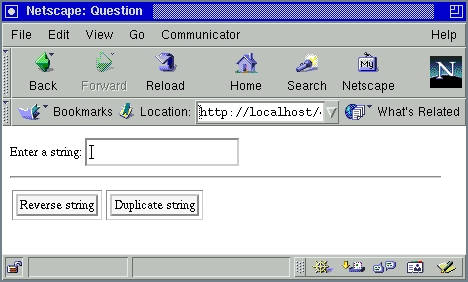
\includegraphics[scale=0.8]{PICTURES/revdup.jpg}
\end{center}\vspace{-3ex}
\caption{A simple string reverse/duplication form\label{fig-revdup}}
\end{figure}
%
\begin{curry}
rdForm :: IO HtmlForm
rdForm = return $ form "Question"
           [htxt "Enter a string: ", textfield tref "", hrule,
            button "Reverse string"   revhandler,
            button "Duplicate string" duphandler]
 where
   tref free

   revhandler env = return $ form "Answer"
     [h1 [htxt $ "Reversed input: " ++ reverse (env tref)]]

   duphandler env = return $ form "Answer"
     [h1 [htxt $ "Duplicated input: " ++ env tref ++ env tref]]
\end{curry} %$
%
Note the simplicity of retrieving values entered into the form:
since the event handlers are called with the appropriate environment
containing these values (parameter \ccode{env}),
they can easily access these values
by applying the environment to the appropriate CGI reference,
like \ccode{(env tref)}.


\section{Further Examples for Web Server Programming}

Now we have seen all elements for writing CGI programs
in Curry.
In this section we will show by various examples how to use
this programming interface. We will see that this programming model
(i.e., logic variables for CGI references,
associated event handlers depending on CGI environments)
is sufficient to solve typical problems in web server programming
in an appropriate way, like
handling sequences of interactions or
holding intermediate states between interactions.


\subsection{Interaction Sequences}

In the previous example, the interaction between the
client and the web server is quite simple:
the client sends a request by filling a form which is answered
by the server with an HTML document containing the requested
information. In realistic applications, it is often the case
that the interaction is not finished by sending back the requested
information but the client requests further (e.g., more detailed)
information based on the received results. Thus, one
has to deal with sequences of longer interactions between the
client and the server.

Our programming model provides a direct support for
interaction sequences. Since the answer provided by the event handler
is an HTML form rather than an HTML expression,
this answer can also contain further input elements
and associated event handlers. By nesting event handlers,
it is straightforward to implement bounded sequences of interactions.
An example for this technique is shown in the next section.

A more interesting question is how to implement
other control abstractions like arbitrary loops.
For this purpose, we show the implementation of a simple
number guessing game: the client has to guess a number
known by the server (here: \code{42}), and for each number entered
by the client the server responds whether this number
is right, smaller or larger than the number to be guessed.
If the guess is not right, the answer form contains an input
field where the client can enter the next guess.
Moreover, the number of guesses should also be counted
and shown at the end.

As the typical approach in declarative languages,
we implement looping constructs by recursion.
Thus, the event handler computing the answer for the client
contains a recursive call to the initial form
which implements the interaction loop.
The entire implementation of this number guessing game
is as follows \proghref{guess}{Program}:
%
\begin{curry}
guessForm :: IO HtmlForm
guessForm = return \$ form "Number Guessing" (guessInput 1)

guessInput :: Int -> [HtmlExp]
guessInput n =
  [htxt "Guess a natural number: ", textfield nref "",
   button "Check" (guessHandler n nref)]   where nref free

guessHandler :: Int -> CgiRef -> (CgiRef -> String) -> IO HtmlForm
guessHandler n nref env =
  return $ form "Answer" $
    case reads (env nref) of
      [(nr,"")] ->
            if nr==42
              then [h1 [htxt $ "Right! You needed "++show n++" guesses!"]]
              else [h1 [htxt $ if nr<42 then "Too small!"
                                        else "Too large!"],
                    hrule] ++ guessInput (n+1)
      _ -> [h1 [htxt "Illegal input, try again!"]] ++ guessInput n
\end{curry}
%
\ccode{guessInput n} is an HTML expression corresponding to
the initial form which contains an
input field for entering the client's guess.
\ccode{guessHandler} is the associated event handler where the
number of guesses and the
CGI reference to the input field are the first and the second argument
of the handler, respectively.
It checks the number entered by the client
(\code{reads}\pindex{reads} is defined in the standard prelude
and used to parse a string into a value)
and returns the different answers depending on the client's guess.
If the guess is not right, the \code{guessInput} is appended
to the answer which implements the recursive call.


\subsection{Handling Intermediate States}
\label{sec-intermediate-state}

A nasty problem in many CGI applications is the handling
of intermediate states due to the fact that HTTP is a stateless
protocol. For instance, in electronic commerce applications,
the clients have shopping baskets where
the already selected items are stored, and the contents of
these baskets must be kept between the interactions.
Storing this information on the server side
has several drawbacks. For instance, the client
wants to identify himself only after he really orders
the items, i.e., during the selection phase the server
cannot uniquely associate the selections to a client.
Furthermore, the client might not proceed with his selections
so that the server does not know whether
the basket information can be deleted (which is necessary
at some point to avoid a memory overflow).
Therefore, it is often better to store such client-dependent
information on the client side. For this purpose,
one can have HTML forms with input elements of type \ccode{hidden}
which have no visual representation but can be used
to pass client-dependent information between interactions.
``Raw'' HTML/CGI programmers must explicitly handle
these fields which is awkward and a source of many
programming problems.

Our programming model offers a much simpler solution
to this problem. By nesting event handlers
(which is allowed in languages with lexical scoping like Curry),
one can directly refer to input elements in previous forms.
As a concrete example, we consider
a sequence of HTML forms where the client enters
his first name in the first form and his last name in the second form.
The complete name is returned in the third form.
This example can be implemented as follows
\proghref{state}{Program}:
%
\begin{curry}
nameForm = return $ form "First Name Form"
  [htxt "Enter your first name: ", textfield firstref "",
   button "Continue" fhandler]
 where
   firstref free

   fhandler _ = return $ form "Last Name Form"
                  [htxt "Enter your last name: ", textfield lastref "",
                   button "Continue" lhandler]
     where
       lastref free

       lhandler env = return $ form "Answer"
                        [htxt $ "Hi, " ++ env firstref ++ " " ++ env lastref]
\end{curry}
%
Due to lexical scoping, the variable \ccode{firstref}
is visible in the event handler \ccode{lhandler} without explicitly
passing it as an argument.


\subsection{Storing Information on the Server}

We have seen how we can retrieve information from the server
by CGI programs. This is possible by performing I/O actions
on the server before computing the HTML form as the response to
the client. In many applications, clients also want to store
or update information on the server, e.g., by putting orders
for books, flight tickets, etc.
In this section we will see a small example that demonstrates
how this can be done using the already known techniques.

Consider the implementation of a web form that counts
and shows the number of visitors. Thus, each visitor
updates the current visitor counter on the server.
This can be easily implemented by storing the current
visitor number in a file.
For this purpose, we define an I/O action \ccode{incVisitNumber}
that reads the number stored in this file, increments it,
stores the incremented number
in the file, and returns the incremented number
(\code{doesFileExist}\pindex{doesFileExist},
\code{removeFile}\pindex{removeFile}, and
\code{renameFile}\pindex{renameFile} are
I/O operations defined in the library \code{Directory}
to check the existence of a file, delete a file, and
rename a file, respectively):\label{sec-overwriteVisitFile}
%
\begin{curry}
incVisitNumber :: IO Int
incVisitNumber = do
 existnumfile <- doesFileExist visitFile
 if existnumfile
   then do vfcont <- readFile visitFile
           overwriteVisitFile (read vfcont + 1)
   else do writeFile visitFile "1"
           return 1

overwriteVisitFile :: Int -> IO Int
overwriteVisitFile n = do
  writeFile (visitFile++".new") (show n)
  removeFile visitFile
  renameFile (visitFile ++ ".new") visitFile
  return n

visitFile :: String
visitFile = "numvisit"  -- file to store the current visitor number
\end{curry}
%
Note the definition of \code{overwriteVisitFile}:
it does not directly write the incremented number
into the \code{visitFile} but it writes it into another file that is
subsequently renamed to the \code{visitFile}.
This is necessary to avoid the overlapping of reading and writing actions
on the same file due to the lazy evaluation of \code{readFile}.

Now the visitor form is simply obtained by calling \code{incVisitNumber}
before generating the form
\proghref{visitor}{Program}:
%
\begin{curry}
visitorForm = do
  visitnum <- incVisitNumber
  return $ form "Access Count Form"
           [h1 [htxt $ "You are the " ++ show visitnum ++ ". visitor!"]]
\end{curry}


\subsection{Ensuring Exclusive Access}
\label{sec-exclusiveIO}

Since CGI programs are executed whenever a client accesses them,
one has not much control on the order of their execution.
In particular, the same CGI program can be executed
in parallel if two clients accessing them simultaneously.
This can cause a problem if both update the same information.
For instance, an access to the visitor form above
reads the current visitor number from the global \code{visitFile}
and write the incremented number back.
If the script is simultaneously executed by two clients,
it may be the case that one update is lost (if both read the same
number and write the same incremented number).

Multiple simultaneous accesses or updates can be avoided
by ensuring the exclusive access to a resource on the web server
between different processes running on the server.
Although Curry has no direct features to support this,\footnote{%
It could be implemented in Curry by the use of ports but this
will be discussed later.}
it can be implemented by the use of the underlying
operating system. For instance, Unix/Linux systems
offer the command \ccode{lockfile} to ensure
an exclusive access to a resource of the system.
\code{lockfile} tries to create
a given file (the argument to \code{lockfile}).
If the file cannot be created (since it has been already created
by another process), the \code{lockfile} command waits
and retries after some time.
Using \code{lockfile}, we can implement a generic function
\ccode{exclusiveIO} that takes a name for a global lock file
and exclusively executes an I/O action (the second parameter),
i.e., it ensures that two processes using the same lock file
do not execute the action at the same time:
%
\begin{curry}
exclusiveIO :: String -> IO a -> IO a
exclusiveIO lockfile action = do
  system ("lockfile " ++ lockfile)
  actionResult <- action
  system ("rm -f " ++ lockfile)
  return actionResult
\end{curry}
%
Now it is straightforward to extend our visitor form
in order to ensure the exclusive update of the visitor counter.
This is done by replacing the expression \code{incVisitNumber}
in the definition of \code{visitorForm} by the following
expression \proghref{exclusive}{Program}:
%
\begin{curry}
exclusiveIO (visitFile ++ ".lock") incVisitNumber
\end{curry}


\subsection{Example: A Web Questionnaire}

\begin{figure}[t]
\begin{center}
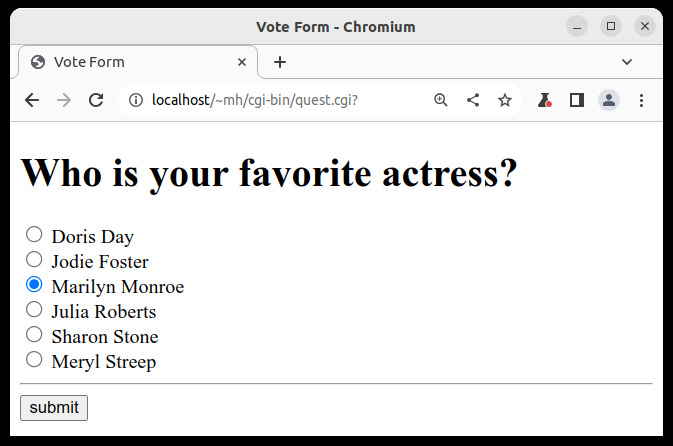
\includegraphics[scale=0.8]{PICTURES/quest.jpg}
\end{center}\vspace{-3ex}
\caption{A web questionnaire\label{fig-quest}}
\end{figure}

This section shows an example for web programming
where the formerly discussed techniques are applied.
Consider the implementation of a web-based questionnaire
which allows the clients to vote on a particular topic.
Figure~\ref{fig-quest} shows an example of such a questionnaire.
The votes are stored on the web server.
The current votings are shown after a client
submits a vote (see Figure~\ref{fig-quest-answer}).

\begin{figure}[t]
\begin{center}
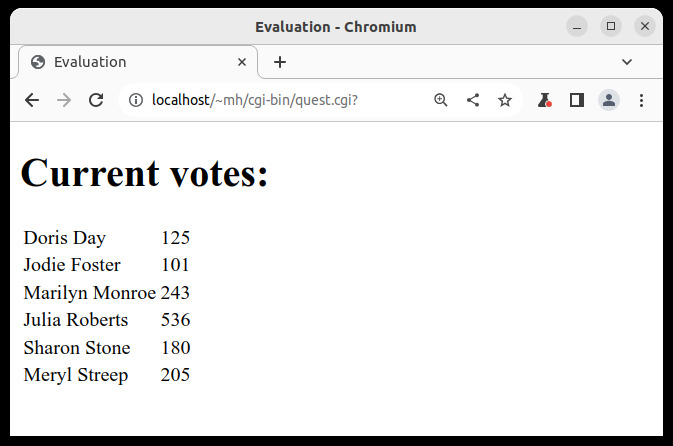
\includegraphics[scale=0.8]{PICTURES/quest_answer.jpg}
\end{center}\vspace{-3ex}
\caption{Answer to the web questionnaire\label{fig-quest-answer}}
\end{figure}

In order to provide an implementation that is easy to maintain,
we define the main question and the choices for the answers
as constants in our program so that they can be easily adapted
to other questionnaires:
\begin{curry}
question = "Who is your favorite actress?"

choices = ["Doris Day", "Jodie Foster", "Marilyn Monroe",
           "Julia Roberts", "Sharon Stone", "Meryl Streep"]
\end{curry}
%
The current votes are stored in a file on the web server.
We define the name of this file as a constant in our program:
%
\begin{curry}
voteFile = "votes.data"
\end{curry}
%
For the sake of simplicity, this file is a simple text file.
If there are $n$ choices for voting, the file has $n$ lines
where each line contains the textual representation of the
number of votes for the corresponding choice.
Thus, the following function defines an action that reads
the vote file and returns the list of numbers in this file
(the prelude function \code{lines}\pindex{lines} breaks
a string into a list of lines where lines are separated by newline
characters):
%
\begin{curry}
readVoteFile :: IO [Int]
readVoteFile = do
  vfcont <- readFile voteFile
  return (map read (lines vfcont))
\end{curry}
%
To initialize the vote file, we define an action \code{initVoteFile}
that initializes the vote file with \code{n} zeros if it does not exist.
The prelude function \code{unlines}\pindex{unlines}
is the opposite of \code{lines} and concatenates a list of strings
into one string by inserting newline characters.
%
\begin{curry}
initVoteFile :: Int -> IO ()
initVoteFile n = do
  existnumfile <- doesFileExist voteFile
  unless existnumfile $
    writeFile voteFile (unlines (map show (take n (repeat 0))))
\end{curry} %$
%
To update the vote file, we define \code{overwriteVoteFile}
that writes a list of
numbers into the vote file. Similarly to the definition of
\code{overwriteVisitFile} in Section~\ref{sec-overwriteVisitFile},
the numbers are written into a new file that is moved to the vote file
in order to avoid an overlapping between reading and writing the same file.
%
\begin{curry}
overwriteVoteFile :: [Int] -> IO ()
overwriteVoteFile nums = do
  writeFile (voteFile ++ ".new") (unlines (map show nums))
  removeFile voteFile
  renameFile (voteFile ++ ".new") voteFile
\end{curry}
%
When a client submits a vote, we have to increment to corresponding
number in the vote file. This can be easily done by a sequence of
actions that initialize the vote file (if necessary), read the current
votes and write the votes that are incremented by the function
\code{incNth}:
\begin{curry}
incNumberInFile :: Int -> IO ()
incNumberInFile n = do
  initVoteFile (length choices)
  nums <- readVoteFile
  overwriteVoteFile (incNth nums n)

incNth :: [Int] -> Int -> [Int]
incNth []     _ = []
incNth (x:xs) n | n==0      = (x+1) : xs
                | otherwise = x : incNth xs (n-1)
\end{curry}
%
Now we have all auxiliary definitions that are necessary to define
the web script. First, we show the definition of
the HTML form \ccode{evalForm} that shows the current votes
(which produces the result shown in Figure~\ref{fig-quest-answer}).
Note that we ensure the exclusive access to the vote file
by the use of the function \ccode{exclusiveIO} defined in
Section~\ref{sec-exclusiveIO}
(the prelude function \ccode{zip}\pindex{zip} joins two lists
into one list of pairs of corresponding elements):
\begin{curry}
evalForm :: IO HtmlForm
evalForm = do
  votes <- exclusiveIO (voteFile ++ ".lock") readVoteFile
  return $ form "Evaluation"
   [h1 [htxt "Current votes:"],
    table (map (\(s,v) -> [[htxt s], [htxt $ show v]])
               (zip choices votes))]
\end{curry}
%
Now we can define our main form that allows the user to submit a
vote (see Figure~\ref{fig-quest}).
It uses radio buttons as input elements.
\label{radio button}\index{button!radio}
Radio buttons are lists of buttons where exactly one button
can be turned on. Thus, all buttons have the same CGI reference
but different values. When a form is submitted, the CGI environment
maps the CGI reference to the value of the selected radio button.
A complete radio button suite consists always of a main button
(\code{radio_main}) which is initially on and some further buttons
with the same CGI reference as the main button (\code{radio_others})
that are initially off.
In our example, we associate to each button the index of the corresponding
choice as a value. The event handler \code{questHandler}
increments he appropriate vote number and returns the current votes
with the form \code{evalForm}
\proghref{questionnaire}{Program}:
\begin{curry}
questForm = return $ form "Vote Form" $
  [h1 [htxt question],
   radio_main vref "0", htxt (' ':head choices), breakline] ++
  concatMap (\(i,s) -> [radio_other vref (show i), htxt (' ':s), breakline])
            (zip [1..] (tail choices)) ++
  [hrule, button "submit" questHandler]
 where
   vref free

   questHandler env = do
     exclusiveIO (voteFile ++ ".lock") (incNumberInFile (read (env vref)))
     evalForm
\end{curry}


\section{Finding Bugs}

Since debugging of CGI programs can be quite tedious,
here are some hints on how to debug CGI programs.

If the execution of the CGI program produces some run-time error
(e.g., access to a non-existing files), the error message
should be shown in the web page.
Furthermore, messages written to standard error output
are collected in the log file of the web script.
For instance, if the web script is stored at location
\code{cgi-bin/myscript.cgi},
the log file is \code{cgi-bin/myscript.cgi.log}.
Hence, if you want to put some debug output in your web script,
you should write it to standard error, e.g.,
%
\begin{curry}
hPutStrLn stderr "A log message"
\end{curry}
%
(where \code{hPutStrLn} and \code{stderr} are defined
in the standard library \code{IO}).

% If the execution of the CGI program does not produce a run-time error
% but simply fails (e.g., because of an incompletely defined function
% are a unification failure), you will probably see the message
% \ccode{No more solutions} in the web browser instead of the
% expected HTML document. For the purpose of debugging,
% it is often useful to see the subexpressions where a
% reduction was not possible but failed. In this case,
% you can  generate the CGI program by \ccode{makecurrycgi}\pindex{makecurrycgi}
% with the option \ccode{-debug}.
% This has the effect that some debugging code is inserted in the CGI
% program so that you can see the trace of all failed subexpressions
% in the browser (not formatted with HTML so that you should better
% view the source with your browser). Note that the debug option
% produces less efficient CGI programs so that it is better to
% use this option only when necessary.

The use of logic variables as references to input elements
in HTML forms ensures that typos in the name of references
can be detected by the compiler (e.g., resulting in an
``undeclared identifier'' error message), in contrast
to traditional approaches to CGI programming using plain strings
as references.
However, if we use the same logic variable for two different
input elements, this is not detected by the compiler
(which is not worse than traditional approaches where this
is also not detected) but results in a run-time error
that is not easy to understand due to the implementation
of the library \code{HTML.Base} in Curry.
In this case, the web script might fail with a message like
\ccode{No value found}.
Thus, you should check your source program for these possible errors
or add some debug output, as described above, to your script.


\section{Advanced Web Programming}
\label{sec-advanced-web-programming}

This section discusses some further features which are useful
for writing web applications in Curry.
\emph{Cookies} are useful to store information about the client
between different web scripts.
\emph{URL parameters} can be exploited to write generic web scripts.
\emph{Style sheets} can be used to modify and add new presentation styles
for web documents.


\subsection{Cookies}

Cookies\index{cookie} are small pieces of information
(represented by strings) that are stored on the client's machine
when a client communicates to a web server via his browser.
The web server can sent cookies to the client together
with a requested web document. If the client wants to retrieve
the same or another document from the web server, the client's browser
sends the stored cookies together with the request for a document
to the browser.
Thus, cookies can be used to identify the client during a longer
interaction with the web server (also across various web scripts
stored on the same web browser).
Cookies are another approach to handle intermediate state
in web applications. The technique presented in
Section~\ref{sec-intermediate-state} is only useful
inside the same web script whereas cookies can be used
as a link between different web scripts.
However, cookies need special support on the browser's side
and the client must enable cookies in his web browser.
Fortunately, most web browsers support cookies
since they are used in many web sites.

Basically, a cookie has a name and a value.
Both parameters are of type string.
Cookies can also have additional parameters to control their
lifetime, validity for different web servers or regions
on a web server etc (see definition of datatype
\ccode{CookieParam} in the library \code{HTML.Base}) which we will not describe
here. As the default, a cookie is a valid during the client's
browser session for all documents in the same directory or
a subdirectory in which the cookie was set.

The library \code{HTML.Base} provides two functions to set
and retrieve cookies.
As described above, a cookie is set by sending it with some
web document. For doing so, there is the function\pindex{cookieForm}
%
\begin{curry}
cookieForm :: String -> [(String,String)] -> [HtmlExp] -> HtmlForm
\end{curry}
%
which behaves similarly to the function \ccode{form} but
takes an additional parameter: a list of cookies, i.e.,
name/value pairs. These cookies are submitted with the form
to the client's browser. To retrieve cookies (that are previously sent
with a \ccode{cookieForm}), there is an I/O action\pindex{getCookies}
%
\begin{curry}
getCookies :: IO [(String,String)]
\end{curry}
%
that returns the list of all cookies (i.e., name/value pairs)
sent from the browser for the current CGI script.

As a simple example, we want to use cookies to write a web application
where a user must identify himself and this identification is used
in another independent script. The identification is done
by setting a cookie of the form \code{("LOGINNAME",<name>)}
where \code{<name>} is the user's name.
We implement a ``login form'' that sets this cookie as follows
\proghref{logincookie}{Program}:
\begin{curry}
loginForm = return $ form "Login"
  [htxt "Enter your name: ", textfield tref "",
   hrule,
   button "Login" handler
  ]
 where
   tref free

   handler env = return $
     cookieForm "Logged In"
                [("LOGINNAME",env tref)]
                [h2 [htxt \$ env tref ++ ": thank you for visiting us"]]
\end{curry}
The first form asks the user for his name.
The cookie is set together with the acknowledgment form
(function \ccode{handler}).

Now we can write another web script that uses this cookie.
This script shows the user's name or the string
\code{"Not yet logged in"} if the user has not used the
login form to set the cookie.
Using the function \code{getCookies}, the implementation
is quite simple (the function \code{lookup}\pindex{lookup}, defined in the
prelude, searches for a name in a name/value list;
it returns \ccode{Nothing} of the name was not found and
\ccode{Just v} if the first occurrence of the name in the list
has the associated value \code{v}; the prelude function
\code{maybe}\pindex{maybe} processes these two cases)
\proghref{logincookie}{Program}:
\begin{curry}
getNameForm = do
  cookies <- getCookies
  return $ form "Hello" $
   maybe [h1 [htxt "Not yet logged in"]]
         (\n -> [h1 [htxt $ "Hello, " ++ n]])
         (lookup "LOGINNAME" cookies)
\end{curry} %$
%
As mentioned above, cookies need special support on the client's
side, i.e., the web browser of the client must support cookies.
If cookies are essential for an application, one should check
whether the client allows the setting of cookies.
This can be done by trying to set a cookie and by checking
whether this was successful. For instance, one can modify
the above login script as folllows.
The first form immediately sets a cookie with name \ccode{SETCOOKIE}.
Then the handler checks whether this cookie has been sent by the
client's browser. If this cookie is not received, it returns a form
with the message ``Sorry, can't set cookies.'' instead of the
acknowledgment form which sets the cookie \ccode{LOGINNAME}
\proghref{checkcookie}{Program}:
\begin{curry}
loginForm = return $ cookieForm "Login" [("SETCOOKIE","")]
  [htxt "Enter your name: ", textfield tref "",
   hrule,
   button "Login" handler
  ]
 where
   tref free

   handler env = do
     cookies <- getCookies
     return $
       if lookup "SETCOOKIE" cookies == Nothing
         then form "No cookies" [h2 [htxt "Sorry, can't set cookies."]]
         else cookieForm "Logged In"
                         [("LOGINNAME", env tref)]
                         [h2 [htxt $ env tref ++ ": thank you for visiting us"]]
\end{curry} %$


\subsection{URL Parameters}

In some situations it is preferable to have generic web scripts that
can be applied in various situations described by parameters.
For instance, if we want to write a web application that
allows the navigation through a hierarchical structure,
one does not want to write a different script for each different
level of the structure but it is preferable to write a single
script that can be applied to different points in the structure.
This is possible by attaching a parameter (a string)
to the URL of a script. For instance, a URL can have the form
\ccode{http://myhost/script.cgi?parameter} where
\ccode{http://myhost/script.cgi} is the URL of the web script
and \ccode{parameter} is an optional parameter that is passed
to the script.
A \emph{URL parameter}\index{URL!parameter}\index{parameter!URL}
can be retrieved inside a script
by the I/O action\pindex{getUrlParameter}
%
\begin{curry}
getUrlParameter :: IO String
\end{curry}
%
which returns the part of the URL following the character \ccode{?}.
Note that an URL parameter should be ``URL encoded'' to avoid
the appearance of characters with a special meaning.
The library \code{HTML.Base} provides the functions
\code{urlencoded2string} and \code{string2urlencoded}
to decode and encode such parameters, respectively.

As a simple example, we want to write a web script to navigate
through a directory structure. The current directory
is the URL parameter for this script. The script
extracts this parameter by the use of \code{getUrlParameter}
and shows all entries as a HTML list
\proghref{browsedir}{Program}
(the prelude function \code{mapM}\pindex{mapM} applies
a mapping from elements into actions to all elements of a list
and collect all results in a list):
%
\begin{curry}
showDirForm = do
  param <- getUrlParameter
  let dir = if param=="" then "." else urlencoded2string param
  entries <- getDirectoryContents dir
  hexps <- mapM (entry2html dir) entries
  return $ form "Browse Directory"
                [h1 [htxt $ "Directory: " ++ dir], ulist hexps]
\end{curry}
%
The I/O action \code{getDirectoryContents}\pindex{getDirectoryContents}
is defined in the system library \code{Directory}
and returns the list of all entries in a directory.
The function \code{entry2html} checks for an entry whether it
is a directory. If this is the case, it returns a link to
the same web script but with an extended parameter, otherwise
it simply returns the entry name as an HTML text
(\code{doesDirectoryExist}\pindex{doesDirectoryExist}
is defined in the library \code{Directory} and returns \code{True}
if the argument is the name of a directory):
%
\begin{curry}
entry2html :: String -> String -> IO [HtmlExp]
entry2html dir e = do
  direx <- doesDirectoryExist (dir ++ "/" ++ e)
  if direx
   then return [href ("browsedir.cgi?" ++ string2urlencoded (dir ++ "/" ++ e))
                     [htxt e]]
   else return [htxt e]
\end{curry}
%


\subsection{Style Sheets}

\todo{To be completed.}


%%% Local Variables: 
%%% mode: latex
%%% TeX-master: "main_pdf"
%%% End: 
% LocalWords:  HTML CGI URL
